% Options for packages loaded elsewhere
% Options for packages loaded elsewhere
\PassOptionsToPackage{unicode}{hyperref}
\PassOptionsToPackage{hyphens}{url}
\PassOptionsToPackage{dvipsnames,svgnames,x11names}{xcolor}
%
\documentclass[
  a4paper,
  DIV=11,
  numbers=noendperiod]{scrreprt}
\usepackage{xcolor}
\usepackage[top=25mm,bottom=25mm,left=20mm,right=20mm]{geometry}
\usepackage{amsmath,amssymb}
\setcounter{secnumdepth}{-\maxdimen} % remove section numbering
\usepackage{iftex}
\ifPDFTeX
  \usepackage[T1]{fontenc}
  \usepackage[utf8]{inputenc}
  \usepackage{textcomp} % provide euro and other symbols
\else % if luatex or xetex
  \usepackage{unicode-math} % this also loads fontspec
  \defaultfontfeatures{Scale=MatchLowercase}
  \defaultfontfeatures[\rmfamily]{Ligatures=TeX,Scale=1}
\fi
\usepackage[]{Verdana}
\ifPDFTeX\else
  % xetex/luatex font selection
\fi
% Use upquote if available, for straight quotes in verbatim environments
\IfFileExists{upquote.sty}{\usepackage{upquote}}{}
\IfFileExists{microtype.sty}{% use microtype if available
  \usepackage[]{microtype}
  \UseMicrotypeSet[protrusion]{basicmath} % disable protrusion for tt fonts
}{}
\makeatletter
\@ifundefined{KOMAClassName}{% if non-KOMA class
  \IfFileExists{parskip.sty}{%
    \usepackage{parskip}
  }{% else
    \setlength{\parindent}{0pt}
    \setlength{\parskip}{6pt plus 2pt minus 1pt}}
}{% if KOMA class
  \KOMAoptions{parskip=half}}
\makeatother
% Make \paragraph and \subparagraph free-standing
\makeatletter
\ifx\paragraph\undefined\else
  \let\oldparagraph\paragraph
  \renewcommand{\paragraph}{
    \@ifstar
      \xxxParagraphStar
      \xxxParagraphNoStar
  }
  \newcommand{\xxxParagraphStar}[1]{\oldparagraph*{#1}\mbox{}}
  \newcommand{\xxxParagraphNoStar}[1]{\oldparagraph{#1}\mbox{}}
\fi
\ifx\subparagraph\undefined\else
  \let\oldsubparagraph\subparagraph
  \renewcommand{\subparagraph}{
    \@ifstar
      \xxxSubParagraphStar
      \xxxSubParagraphNoStar
  }
  \newcommand{\xxxSubParagraphStar}[1]{\oldsubparagraph*{#1}\mbox{}}
  \newcommand{\xxxSubParagraphNoStar}[1]{\oldsubparagraph{#1}\mbox{}}
\fi
\makeatother

\usepackage{color}
\usepackage{fancyvrb}
\newcommand{\VerbBar}{|}
\newcommand{\VERB}{\Verb[commandchars=\\\{\}]}
\DefineVerbatimEnvironment{Highlighting}{Verbatim}{commandchars=\\\{\}}
% Add ',fontsize=\small' for more characters per line
\usepackage{framed}
\definecolor{shadecolor}{RGB}{241,243,245}
\newenvironment{Shaded}{\begin{snugshade}}{\end{snugshade}}
\newcommand{\AlertTok}[1]{\textcolor[rgb]{0.68,0.00,0.00}{#1}}
\newcommand{\AnnotationTok}[1]{\textcolor[rgb]{0.37,0.37,0.37}{#1}}
\newcommand{\AttributeTok}[1]{\textcolor[rgb]{0.40,0.45,0.13}{#1}}
\newcommand{\BaseNTok}[1]{\textcolor[rgb]{0.68,0.00,0.00}{#1}}
\newcommand{\BuiltInTok}[1]{\textcolor[rgb]{0.00,0.23,0.31}{#1}}
\newcommand{\CharTok}[1]{\textcolor[rgb]{0.13,0.47,0.30}{#1}}
\newcommand{\CommentTok}[1]{\textcolor[rgb]{0.37,0.37,0.37}{#1}}
\newcommand{\CommentVarTok}[1]{\textcolor[rgb]{0.37,0.37,0.37}{\textit{#1}}}
\newcommand{\ConstantTok}[1]{\textcolor[rgb]{0.56,0.35,0.01}{#1}}
\newcommand{\ControlFlowTok}[1]{\textcolor[rgb]{0.00,0.23,0.31}{\textbf{#1}}}
\newcommand{\DataTypeTok}[1]{\textcolor[rgb]{0.68,0.00,0.00}{#1}}
\newcommand{\DecValTok}[1]{\textcolor[rgb]{0.68,0.00,0.00}{#1}}
\newcommand{\DocumentationTok}[1]{\textcolor[rgb]{0.37,0.37,0.37}{\textit{#1}}}
\newcommand{\ErrorTok}[1]{\textcolor[rgb]{0.68,0.00,0.00}{#1}}
\newcommand{\ExtensionTok}[1]{\textcolor[rgb]{0.00,0.23,0.31}{#1}}
\newcommand{\FloatTok}[1]{\textcolor[rgb]{0.68,0.00,0.00}{#1}}
\newcommand{\FunctionTok}[1]{\textcolor[rgb]{0.28,0.35,0.67}{#1}}
\newcommand{\ImportTok}[1]{\textcolor[rgb]{0.00,0.46,0.62}{#1}}
\newcommand{\InformationTok}[1]{\textcolor[rgb]{0.37,0.37,0.37}{#1}}
\newcommand{\KeywordTok}[1]{\textcolor[rgb]{0.00,0.23,0.31}{\textbf{#1}}}
\newcommand{\NormalTok}[1]{\textcolor[rgb]{0.00,0.23,0.31}{#1}}
\newcommand{\OperatorTok}[1]{\textcolor[rgb]{0.37,0.37,0.37}{#1}}
\newcommand{\OtherTok}[1]{\textcolor[rgb]{0.00,0.23,0.31}{#1}}
\newcommand{\PreprocessorTok}[1]{\textcolor[rgb]{0.68,0.00,0.00}{#1}}
\newcommand{\RegionMarkerTok}[1]{\textcolor[rgb]{0.00,0.23,0.31}{#1}}
\newcommand{\SpecialCharTok}[1]{\textcolor[rgb]{0.37,0.37,0.37}{#1}}
\newcommand{\SpecialStringTok}[1]{\textcolor[rgb]{0.13,0.47,0.30}{#1}}
\newcommand{\StringTok}[1]{\textcolor[rgb]{0.13,0.47,0.30}{#1}}
\newcommand{\VariableTok}[1]{\textcolor[rgb]{0.07,0.07,0.07}{#1}}
\newcommand{\VerbatimStringTok}[1]{\textcolor[rgb]{0.13,0.47,0.30}{#1}}
\newcommand{\WarningTok}[1]{\textcolor[rgb]{0.37,0.37,0.37}{\textit{#1}}}

\usepackage{longtable,booktabs,array}
\usepackage{calc} % for calculating minipage widths
% Correct order of tables after \paragraph or \subparagraph
\usepackage{etoolbox}
\makeatletter
\patchcmd\longtable{\par}{\if@noskipsec\mbox{}\fi\par}{}{}
\makeatother
% Allow footnotes in longtable head/foot
\IfFileExists{footnotehyper.sty}{\usepackage{footnotehyper}}{\usepackage{footnote}}
\makesavenoteenv{longtable}
\usepackage{graphicx}
\makeatletter
\newsavebox\pandoc@box
\newcommand*\pandocbounded[1]{% scales image to fit in text height/width
  \sbox\pandoc@box{#1}%
  \Gscale@div\@tempa{\textheight}{\dimexpr\ht\pandoc@box+\dp\pandoc@box\relax}%
  \Gscale@div\@tempb{\linewidth}{\wd\pandoc@box}%
  \ifdim\@tempb\p@<\@tempa\p@\let\@tempa\@tempb\fi% select the smaller of both
  \ifdim\@tempa\p@<\p@\scalebox{\@tempa}{\usebox\pandoc@box}%
  \else\usebox{\pandoc@box}%
  \fi%
}
% Set default figure placement to htbp
\def\fps@figure{htbp}
\makeatother

\ifLuaTeX
  \usepackage{luacolor}
  \usepackage[soul]{lua-ul}
\else
  \usepackage{soul}
\fi




\setlength{\emergencystretch}{3em} % prevent overfull lines

\providecommand{\tightlist}{%
  \setlength{\itemsep}{0pt}\setlength{\parskip}{0pt}}



 


\KOMAoption{captions}{tableheading}
\makeatletter
\@ifpackageloaded{tcolorbox}{}{\usepackage[skins,breakable]{tcolorbox}}
\@ifpackageloaded{fontawesome5}{}{\usepackage{fontawesome5}}
\definecolor{quarto-callout-color}{HTML}{909090}
\definecolor{quarto-callout-note-color}{HTML}{0758E5}
\definecolor{quarto-callout-important-color}{HTML}{CC1914}
\definecolor{quarto-callout-warning-color}{HTML}{EB9113}
\definecolor{quarto-callout-tip-color}{HTML}{00A047}
\definecolor{quarto-callout-caution-color}{HTML}{FC5300}
\definecolor{quarto-callout-color-frame}{HTML}{acacac}
\definecolor{quarto-callout-note-color-frame}{HTML}{4582ec}
\definecolor{quarto-callout-important-color-frame}{HTML}{d9534f}
\definecolor{quarto-callout-warning-color-frame}{HTML}{f0ad4e}
\definecolor{quarto-callout-tip-color-frame}{HTML}{02b875}
\definecolor{quarto-callout-caution-color-frame}{HTML}{fd7e14}
\makeatother
\makeatletter
\@ifpackageloaded{caption}{}{\usepackage{caption}}
\AtBeginDocument{%
\ifdefined\contentsname
  \renewcommand*\contentsname{Table of contents}
\else
  \newcommand\contentsname{Table of contents}
\fi
\ifdefined\listfigurename
  \renewcommand*\listfigurename{List of Figures}
\else
  \newcommand\listfigurename{List of Figures}
\fi
\ifdefined\listtablename
  \renewcommand*\listtablename{List of Tables}
\else
  \newcommand\listtablename{List of Tables}
\fi
\ifdefined\figurename
  \renewcommand*\figurename{Figure}
\else
  \newcommand\figurename{Figure}
\fi
\ifdefined\tablename
  \renewcommand*\tablename{Table}
\else
  \newcommand\tablename{Table}
\fi
}
\@ifpackageloaded{float}{}{\usepackage{float}}
\floatstyle{ruled}
\@ifundefined{c@chapter}{\newfloat{codelisting}{h}{lop}}{\newfloat{codelisting}{h}{lop}[chapter]}
\floatname{codelisting}{Listing}
\newcommand*\listoflistings{\listof{codelisting}{List of Listings}}
\makeatother
\makeatletter
\makeatother
\makeatletter
\@ifpackageloaded{caption}{}{\usepackage{caption}}
\@ifpackageloaded{subcaption}{}{\usepackage{subcaption}}
\makeatother
\usepackage{bookmark}
\IfFileExists{xurl.sty}{\usepackage{xurl}}{} % add URL line breaks if available
\urlstyle{same}
\hypersetup{
  pdftitle={Introduction to R},
  pdfauthor={Emma James},
  colorlinks=true,
  linkcolor={blue},
  filecolor={Maroon},
  citecolor={Blue},
  urlcolor={Blue},
  pdfcreator={LaTeX via pandoc}}


\title{Introduction to R\thanks{These materials are adapted from an
original version by Dan Baker.}}
\author{Emma James}
\date{}
\begin{document}
\maketitle


\chapter{Introduction}\label{introduction}

The overarching aim of this practical is to get you used to the R
environment. The best way to do this is to start with something you
already know about: basic statistics from your first and second year.
Along the way we will introduce basic concepts common to all programming
languages, with no prior programming knowledge assumed.

\begin{tcolorbox}[enhanced jigsaw, colbacktitle=quarto-callout-note-color!10!white, leftrule=.75mm, breakable, colframe=quarto-callout-note-color-frame, opacityback=0, titlerule=0mm, rightrule=.15mm, opacitybacktitle=0.6, colback=white, coltitle=black, toprule=.15mm, bottomtitle=1mm, bottomrule=.15mm, toptitle=1mm, title={Learning objectives}, arc=.35mm, left=2mm]

By the end of this practical, you will be able to:

\begin{enumerate}
\def\labelenumi{\arabic{enumi}.}
\tightlist
\item
  Use \emph{RStudio} to write, comment, and execute lines of code.
\item
  Create and manipulate objects in \emph{R.}
\item
  Load data files into \emph{R.}
\item
  Calculate basic summary statistics.
\item
  Implement common inferential tests, including a t-test, correlation,
  and ANOVA.
\end{enumerate}

\end{tcolorbox}

\begin{center}\rule{0.5\linewidth}{0.5pt}\end{center}

\chapter{Navigating RStudio and creating
objects}\label{navigating-rstudio-and-creating-objects}

Here is the main window of \emph{RStudio} (shown on a Windows PC,
although it should look very similar on a Mac!). You can see that it has
four different sections.

\begin{figure}[H]

{\centering \pandocbounded{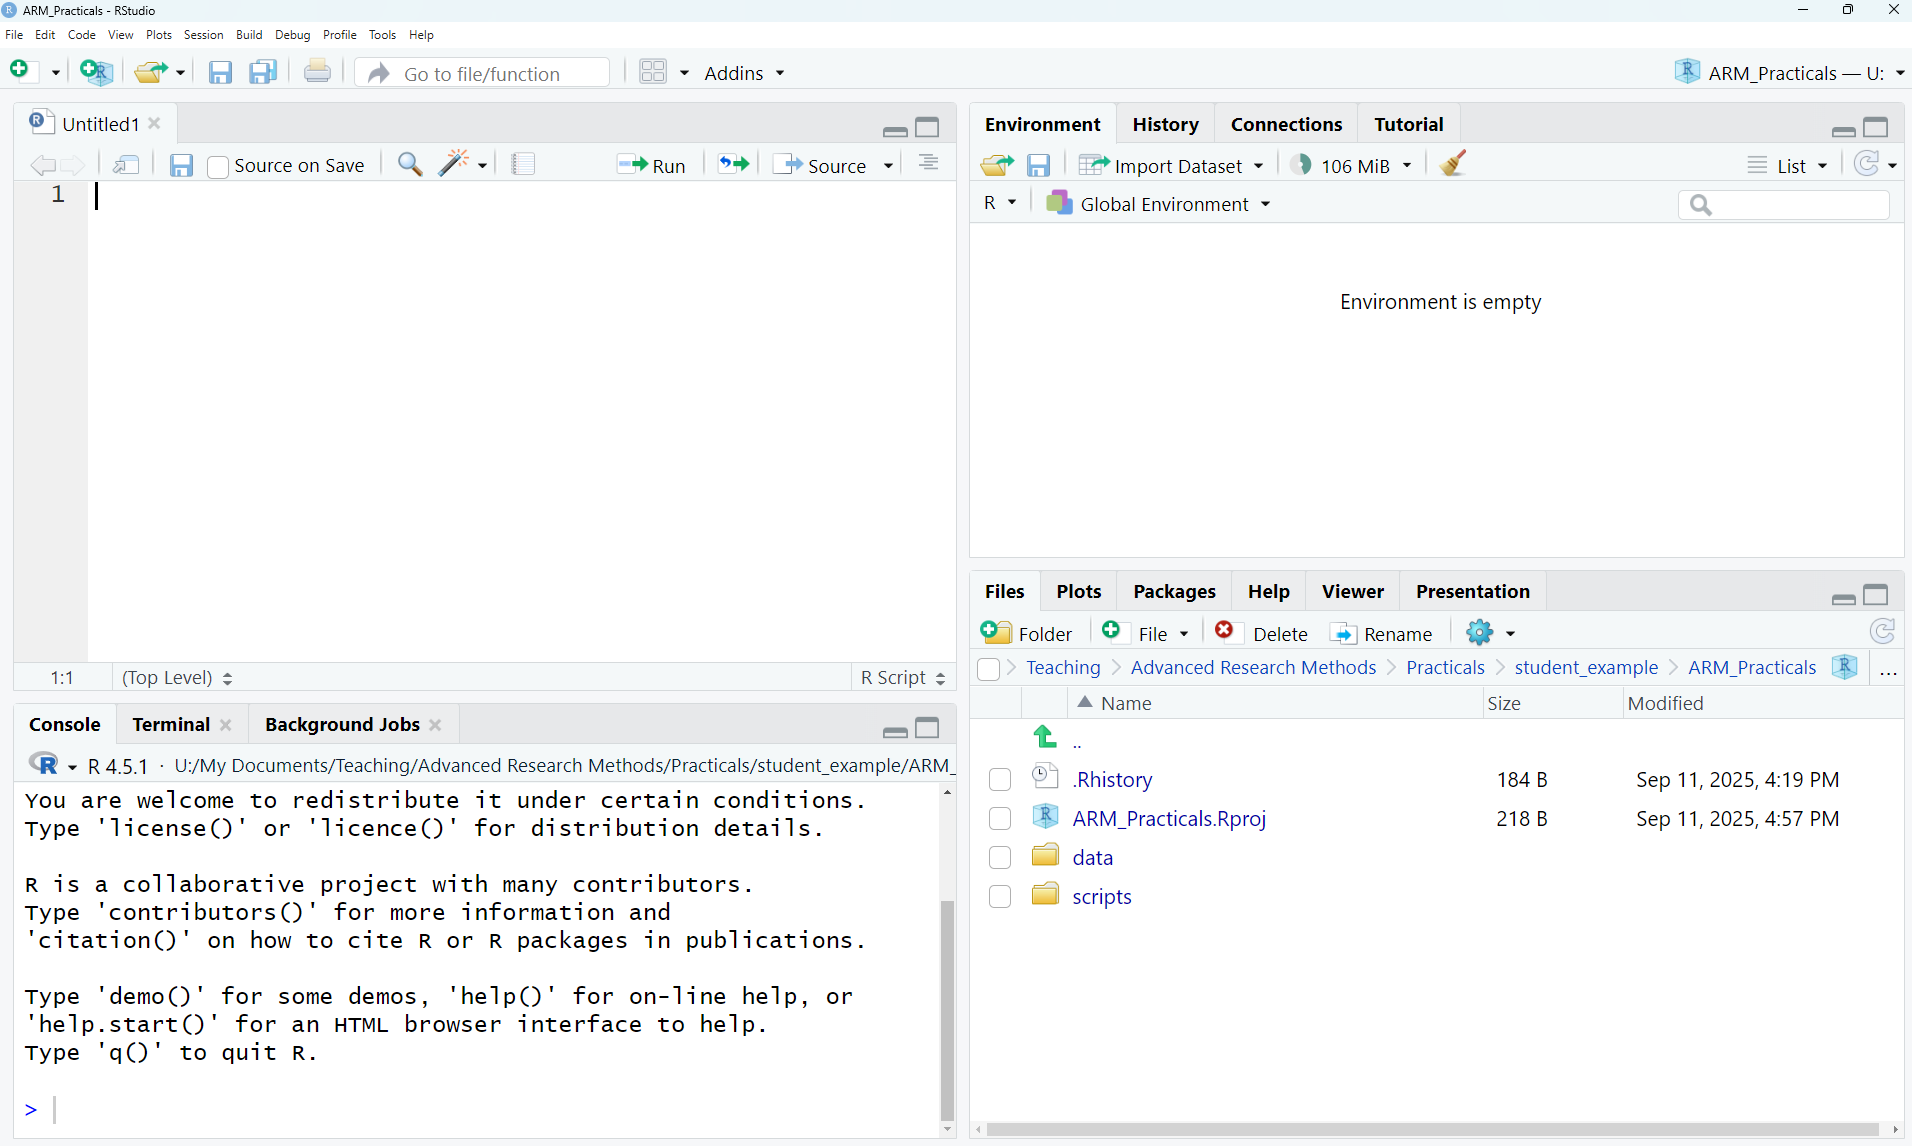
\includegraphics[keepaspectratio]{images/RStudio_window.PNG}}

}

\caption{Default RStudio layout}

\end{figure}%

\section{Top left: Scripts}\label{top-left-scripts}

In the top left corner of the image is a quadrant for your scripts. You
won't see this quadrant when you first open R, but it will show when you
create one in Section 2.

Scripts are like lists of instructions for the computer to follow. You
can save them just like a Word document, and this makes it easy to set
up complex analyses without typing them in by hand each time. Throughout
these practicals, you will create several scripts that you can later
adapt and reuse in running statistical analyses.

\section{Bottom left: Console}\label{bottom-left-console}

The lower left window is called the \emph{Console}. This is where the
magic happens! Here, you can type in individual commands to ask the
computer to do something. You can use it just like a calculator: try
clicking in the console and typing \texttt{20\ +\ 57} (or indeed any
other sum you choose!). If you press the Enter/Return key, you should
see the answer printed below.

We can also instruct the computer to create an ``object'' (or
``variable''\footnote{In programming, ``variables'' are used to store
  information in memory. In \emph{R,} a language used for statistics,
  these are commonly referred to as ``objects'' to avoid confusion with
  the use of ``variable'' in relation to your data (i.e., a column in
  your dataset, your independent/dependent variables). You will see
  these referred to as either, and either is fine.}). An object is like
a box that you can store information in. Some objects are big, such as
large datasets that contain many numbers or even chunks of text. Others
might contain only one number.

First, let's create an object called \texttt{a}, and give it the value
5. Click on the Console area and type:

\begin{Shaded}
\begin{Highlighting}[]
\NormalTok{a }\OtherTok{\textless{}{-}} \DecValTok{5}
\end{Highlighting}
\end{Shaded}

Then hit the Enter/Return key to run it. You will see the arrows
\texttt{\textless{}-} a lot in R: they are used to assign (or store)
everything on the right to the name that you provide on the
left\footnote{If you already have some programming experience, you might
  be more used to using the \texttt{=} symbol to assign values. This
  works fine in \emph{R} too so can be used if you prefer. However,
  using the \texttt{\textless{}-} is more clearly distinguished from
  other aspects of \emph{R} code, and so is more readily used/taught.}.

\section{Top right: Environment}\label{top-right-environment}

If you have created an object, \texttt{a}, you should now see that it
has appeared in the top right section, in the \emph{Environment} tab,
with the assigned value 5. This means that we can now treat \texttt{a}
as though it is a number: we can run mathematical operations on the
object, and get out an answer that depends on the value assigned. You
can try this now by typing \texttt{a*2} into the console to multiply it
by two, or \texttt{a\^{}2} to square it.

So why not just type 5\^{}2 in the first place? The reason objects are
useful is that we can change and update their values, or include many
numbers in them. Let's make a new object called \texttt{b} with the
numbers 1-5, and see what happens when we square it:

\begin{Shaded}
\begin{Highlighting}[]
\NormalTok{b }\OtherTok{\textless{}{-}} \FunctionTok{c}\NormalTok{(}\DecValTok{1}\NormalTok{, }\DecValTok{2}\NormalTok{, }\DecValTok{3}\NormalTok{, }\DecValTok{4}\NormalTok{, }\DecValTok{5}\NormalTok{)}
\NormalTok{b}\SpecialCharTok{\^{}}\DecValTok{2}
\end{Highlighting}
\end{Shaded}

\begin{verbatim}
[1]  1  4  9 16 25
\end{verbatim}

You can see that we now get a list of the squares of all the elements.

We will use objects to store and manipulate data in \emph{R}, similar to
how we might work on a spreadsheet or SPSS file. You can always inspect
the objects you have to hand and the values assigned to them by looking
in the Environment panel.

\section{Bottom right: Other things!}\label{bottom-right-other-things}

The bottom right window has several sections that can be navigated by
clicking on the tabs at the top. \emph{Files} shows the files in the
directory that we are working from, \emph{Plots} will contain any
figures that we create, \emph{Packages} contains a list of extensions
that will enable us to do different types of statistics, and the
\emph{Help} table will show the help pages for a particular function if
we ask for them (we'll do this a lot!).

\begin{center}\rule{0.5\linewidth}{0.5pt}\end{center}

\chapter{Creating a script and loading in
data}\label{creating-a-script-and-loading-in-data}

In this section, we will create a script to tell us about the mean,
median, standard deviation, and standard error of some data. Rather than
type the data in by hand, we will load a dataset from a file---just as
we would if we had run an experiment.

\section{Opening your R Project}\label{opening-your-r-project}

Make sure that you are working in the R Project
\textbf{ARM\_Practicals}. This should be the case if you have just
completed the 0\_SetUp instructions. If not, or if you closed RStudio in
between, you can open this by clicking \emph{File
\textgreater\textgreater{} Open Project\ldots{}} and navigating to the
project file we created.

Remember, you should be able to see this in the top-right corner of the
RStudio window.

\begin{figure}[H]

{\centering \pandocbounded{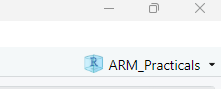
\includegraphics[keepaspectratio]{images/RProject.png}}

}

\caption{Current R Project open}

\end{figure}%

\section{Creating a script}\label{creating-a-script}

Look to the top left of your RStudio window. Click the button that has a
white square and cross in a green circle (or alternatively, click
\emph{File \textgreater\textgreater{} New File
\textgreater\textgreater{} R Script}). Now you have a script open, let's
save it so that we can keep saving our progress as we go. Click
\emph{File \textgreater\textgreater{} Save As\ldots{}} and navigate to
the scripts folder inside the ARM\_Practicals folder you created. Once
you are in this folder, save your script with the name
\textbf{ARM1\_intro.R}.

\section{Loading data into R}\label{loading-data-into-r}

There is a file in the Lecture 1 section of the VLE called
\textbf{ARM1\_data1\_gamers.csv}. This is a .csv file, which is a
readily used data storage format that can be opened by many different
software\footnote{If you wish to read in different file types in the
  future (e.g., .xlsx, .sav), there are many different bespoke packages
  available that will support you in doing this (e.g., read\_excel,
  haven).}. Download this file, and save it in the folder we previously
created (likely \emph{Documents/ARM\_Practicals/data/}).

At the top of your script file, you can now instruct R to read in the
dataset by adding the following line:

\begin{Shaded}
\begin{Highlighting}[]
\NormalTok{gamer\_dat }\OtherTok{\textless{}{-}} \FunctionTok{read.csv}\NormalTok{(}\StringTok{"./data/ARM1\_data1\_gamers.csv"}\NormalTok{)}
\end{Highlighting}
\end{Shaded}

We are creating an object in R here called \texttt{gamer\_dat}, and
using the \texttt{\textless{}-} to assign something to it. Here, we want
to assign the data file that we load in, so need to instruct it to find
and load the data file. We use \texttt{read.csv()} to tell R that we
want to load in a csv file. We tell it the file path to where the
dataset is stored: the \texttt{./} affirms that we are starting in the
current directory (your R project folder), then \texttt{data/} instructs
it to look in the data folder, then the final part is the name of the
file (including the .csv extension).

Now you have typed this into your script, you need to execute it. You
can do this by highlighting it with your mouse and then clicking `Run'
at the top of the script. Alternatively, if your cursor is on the
correct line, you can hit Ctrl + Enter on your keyboard.

If you are successful, you should see an object called
\texttt{gamer\_dat} appear in the \emph{Environment} tab. You can see
that it has 100 observations (rows) for 5 variables (columns). If you
click the little grid to the right of this description, you can inspect
the dataset in your top left panel. You should see that the five columns
correspond to:

\begin{itemize}
\tightlist
\item
  \textbf{ppt\_id}: a unique identifying code for each participant
\item
  \textbf{age\_years}: their age in years
\item
  \textbf{gamer}: whether they play video games (y) or not (n)
\item
  \textbf{hours}: if they do play video games, how many hours they play
  per week on average (or NA if they don't, meaning that it's a missing
  value)
\item
  \textbf{wmc}: working memory capacity
\end{itemize}

\emph{This dataset was simulated for the purposes of today's practical,
but was inspired by a
\href{https://doi.org/10.1016/j.heliyon.2023.e19098}{research study} by
Fiona McNab.}

\begin{center}\rule{0.5\linewidth}{0.5pt}\end{center}

\chapter{Calculating summary
statistics}\label{calculating-summary-statistics}

R has many built in functions to calculate basic descriptive statistics.
Now you have loaded your data, try adding the following line to your
script:

\begin{Shaded}
\begin{Highlighting}[]
\FunctionTok{mean}\NormalTok{(gamer\_dat}\SpecialCharTok{$}\NormalTok{wmc)}
\end{Highlighting}
\end{Shaded}

In this section of code, \texttt{mean()} calls the function to calculate
the mean statistic. Inside the brackets, you need to tell the function
what to calculate the mean of. We've referenced this by using the name
of the object (i.e., the \texttt{gamer\_dat} label we gave the dataset
when we loaded it in), and then used the \texttt{\$} sign to specify
which variable of the object we are interested in (here, \texttt{wmc}).

Now you have typed this into your script, you need to execute it. You
can do this by highlighting it with your mouse and then clicking `Run'
at the top of the script. Alternatively, if your cursor is on the
correct line, you can hit Ctrl + Enter on your keyboard. You should see
that your line of script now appears in the Console, followed by the
answer as follows:

\begin{Shaded}
\begin{Highlighting}[]
\FunctionTok{mean}\NormalTok{(gamer\_dat}\SpecialCharTok{$}\NormalTok{wmc)}
\end{Highlighting}
\end{Shaded}

\begin{verbatim}
[1] 8.43
\end{verbatim}

If it hasn't worked, go back over the previous instructions carefully
and see if you missed a step. The console will contain any error
messages in red. If you are still stuck, raise your hand.

You can calculate some other descriptive statistics, and create a
histogram as follows:

\begin{Shaded}
\begin{Highlighting}[]
\FunctionTok{median}\NormalTok{(gamer\_dat}\SpecialCharTok{$}\NormalTok{wmc)}
\FunctionTok{sd}\NormalTok{(gamer\_dat}\SpecialCharTok{$}\NormalTok{wmc)}
\FunctionTok{sd}\NormalTok{(gamer\_dat}\SpecialCharTok{$}\NormalTok{wmc)}\SpecialCharTok{/}\FunctionTok{sqrt}\NormalTok{(}\FunctionTok{length}\NormalTok{(gamer\_dat}\SpecialCharTok{$}\NormalTok{wmc))}
\FunctionTok{hist}\NormalTok{(gamer\_dat}\SpecialCharTok{$}\NormalTok{wmc)}
\end{Highlighting}
\end{Shaded}

These lines compute the median, standard deviation and standard error,
and then plot a histogram. If you select your entire script and run it,
you will see these values appear in the \emph{Console} and a histogram
of the data appear in the \emph{Plots} window. Well done -- you have
just written your first \emph{R} script!\footnote{The eagle-eyed among
  you might also see that you have your first example of rainbow
  brackets, if you turned on this setting during the 0\_SetUp task!}

\begin{tcolorbox}[enhanced jigsaw, colbacktitle=quarto-callout-tip-color!10!white, leftrule=.75mm, breakable, colframe=quarto-callout-tip-color-frame, opacityback=0, titlerule=0mm, rightrule=.15mm, opacitybacktitle=0.6, colback=white, coltitle=black, toprule=.15mm, bottomtitle=1mm, bottomrule=.15mm, toptitle=1mm, title=\textcolor{quarto-callout-tip-color}{\faLightbulb}\hspace{0.5em}{Take note! (literally)}, arc=.35mm, left=2mm]

Before we go any further, we should talk about good coding practices.
It's very helpful if you can add comments to your code to say what you
are doing in each section. This is helpful as a learner, allowing you
look back at the scripts that we write in these practicals without
having to match it up with this worksheet. It's also good practice as
you write more advanced scripts: future you will be very grateful for
notes explaining what you are doing at each step.

You can add comments to your script by using the \# symbol. When R
encounters the \# symbol, it knows not to try and interpret the
remainder of that line as code. This means that you can either write
comments on their own line or directly next to code, like in the example
below.

Try it now: add comments to the code you have already written so that
future you will remember what this code does. You should try to do this
throughout all the practicals: I have often written basic comments
alongside sections of code, but you can edit these and add more notes to
your scripts to help you to remember key things.

\end{tcolorbox}

\begin{Shaded}
\begin{Highlighting}[]
\CommentTok{\# Calculate descriptive statistics }
\FunctionTok{mean}\NormalTok{(gamer\_dat}\SpecialCharTok{$}\NormalTok{wmc)  }\CommentTok{\# mean }
\FunctionTok{sd}\NormalTok{(gamer\_dat}\SpecialCharTok{$}\NormalTok{wmc)    }\CommentTok{\# standard deviation}
\end{Highlighting}
\end{Shaded}

\begin{center}\rule{0.5\linewidth}{0.5pt}\end{center}

\chapter{Running inferential tests}\label{running-inferential-tests}

\section{Running a t-test}\label{running-a-t-test}

In Years 1 and 2, you learned about some inferential statistics that
test the relationship between two variables.

One way to analyse the data that you have loaded is to run a t-test to
test the difference in means between two groups. Let's test the
hypothesis that gamers versus non-gamers have different working memory
capacity. You can do this by adding the following line of code to your
script:

\begin{Shaded}
\begin{Highlighting}[]
\FunctionTok{t.test}\NormalTok{(wmc }\SpecialCharTok{\textasciitilde{}}\NormalTok{ gamer, }\AttributeTok{data =}\NormalTok{ gamer\_dat)}
\end{Highlighting}
\end{Shaded}

Within the t.test call, we have asked for our dependent variable
(\texttt{wmc}) to be predicted by (\texttt{\textasciitilde{}}) the
variable \texttt{gamer}, which we have seen has two levels (\emph{y,
n}). We don't actually have objects called \texttt{wmc} and
\texttt{gamer} in our R environment, so we specify that it should look
for these within the \texttt{gamer\_dat} dataset.

Running this line of code should give you the following output:

\begin{verbatim}

    Welch Two Sample t-test

data:  wmc by gamer
t = -2.3734, df = 96.462, p-value = 0.01961
alternative hypothesis: true difference in means between group n and group y is not equal to 0
95 percent confidence interval:
 -1.8730152 -0.1669848
sample estimates:
mean in group n mean in group y 
           7.92            8.94 
\end{verbatim}

The output tells us the test that we have run, and provides us with the
necessary values for reporting on the third line of output: the
\emph{t}-statistic, degrees of freedom, and \emph{p-}value. You can see
here that there is a significant difference between the two groups as
the \emph{p} \textless{} .05. The output also handily summarises the
mean working memory capacity for each group.

\section{Running a correlation}\label{running-a-correlation}

Another simple analysis for testing the relationship between two
variables is a correlation, which we can use to test the strength of
association between two continuous variables. Let's test how working
memory capacity changes with age, by typing the following line.

\begin{Shaded}
\begin{Highlighting}[]
\FunctionTok{cor.test}\NormalTok{(}\AttributeTok{formula =} \SpecialCharTok{\textasciitilde{}}\NormalTok{ age\_years }\SpecialCharTok{+}\NormalTok{ wmc, }\AttributeTok{data =}\NormalTok{ gamer\_dat)}
\end{Highlighting}
\end{Shaded}

Running this line of code should produce the following:

\begin{verbatim}

    Pearson's product-moment correlation

data:  age_years and wmc
t = -2.2034, df = 98, p-value = 0.02991
alternative hypothesis: true correlation is not equal to 0
95 percent confidence interval:
 -0.39674850 -0.02177224
sample estimates:
       cor 
-0.2172612 
\end{verbatim}

Again, the output tells us the test that has been done, and shows us
that there is a significant relationship between the two variables
(\emph{p} = 0.02). The final line of output, labelled as ``cor'', is the
correlation coefficient, showing a negative correlation between the two
variables: as age increases, working memory decreases.

These calls for statistical tests that we have just run are called
\emph{functions.} We also used functions above to read in the data, and
gain some summary statistics. You can find out more about the options
available for each function by typing e.g., \texttt{help(t.test)} or
\texttt{help(cor.test)} in the \emph{Console} (this is a bit meta, we
use the \texttt{help()} function to ask for help about other
functions)\emph{.} This should bring up some helpful information in the
bottom right window. The help pages tell you which ``Arguments'' you
need to give to the function, and how to specify them. For example, we
can see that to run a Spearman test rather than a Pearson's correlation,
we should add the argument \texttt{method\ =\ "spearman"} inside the
brackets. Try this now.

\section{Running an ANOVA}\label{running-an-anova}

Finally, let's try running a simple one-way ANOVA. Now you've
established that gamers have a higher working memory capacity than
non-gamers, we might want to ask whether it matters what \emph{type} of
games people are playing. You run a new study and recruit only young
adults who self-report as gamers. You measure their working capacity,
and ask them to select their dominant game type.

Make sure that you have downloaded the data from the VLE and saved it in
your data folder. Then let's load it into R and assign it to an object
called \texttt{type\_dat}. Inspect the dataset to see the game
categories.

\begin{Shaded}
\begin{Highlighting}[]
\NormalTok{type\_dat }\OtherTok{\textless{}{-}} \FunctionTok{read.csv}\NormalTok{(}\StringTok{"./data/ARM1\_data2\_gametype.csv"}\NormalTok{)}
\end{Highlighting}
\end{Shaded}

Given there are three levels of game type, we can no longer use a t-test
to compare working memory between groups. Instead, we can use a one-way
ANOVA.

The first step in running an ANOVA is to check the assumption of
homogeneity of variance using Levene's test. This test isn't included as
standard in R, so we need to load in a package (a set of functions that
someone has written) to run it. You only need to run this once in each R
session. Add the following lines to your script, and run them:

\begin{Shaded}
\begin{Highlighting}[]
\CommentTok{\# Load car package}
\FunctionTok{library}\NormalTok{(car)}

\CommentTok{\# Run Levene\textquotesingle{}s test}
\FunctionTok{leveneTest}\NormalTok{(wmc }\SpecialCharTok{\textasciitilde{}}\NormalTok{ type, }\AttributeTok{data =}\NormalTok{ type\_dat)}
\end{Highlighting}
\end{Shaded}

\begin{verbatim}
Warning in leveneTest.default(y = y, group = group, ...): group coerced to
factor.
\end{verbatim}

\begin{verbatim}
Levene's Test for Homogeneity of Variance (center = median)
      Df F value Pr(>F)
group  2  1.4751 0.2344
      87               
\end{verbatim}

The output prints a warning that it interpreted our group (i.e., game
type) as a factor. This is fine, that's what we want it to do! You can
then see that the test is not significant, so we can assume that the
variances are equal across the groups. This means that we can proceed
with our ANOVA.

We can run the test and display the results using only two lines of
code:

\begin{Shaded}
\begin{Highlighting}[]
\CommentTok{\# Run ANOVA and save output to object}
\NormalTok{gametype\_model }\OtherTok{\textless{}{-}} \FunctionTok{aov}\NormalTok{(wmc }\SpecialCharTok{\textasciitilde{}}\NormalTok{ type, }\AttributeTok{data =}\NormalTok{ type\_dat)}

\CommentTok{\# Print output summary}
\FunctionTok{summary}\NormalTok{(gametype\_model)}
\end{Highlighting}
\end{Shaded}

This will produce your ANOVA summary table as follows:

\begin{verbatim}
            Df Sum Sq Mean Sq F value   Pr(>F)    
type         2  70.42   35.21   11.12 5.01e-05 ***
Residuals   87 275.53    3.17                     
---
Signif. codes:  0 '***' 0.001 '**' 0.01 '*' 0.05 '.' 0.1 ' ' 1
\end{verbatim}

Just like in SPSS, we can pick out the degrees of freedom (2, 87), the F
ratio (4.806) and the \emph{p}-value (.01). Here we can see that there
is a significant difference in working memory capacity depending on the
type of game that people play most regularly (\emph{p} \textless{} .05).

\begin{center}\rule{0.5\linewidth}{0.5pt}\end{center}

\chapter{Summary}\label{summary}

We've just introduced some important concepts in R, and gone through how
to do some basic statistical tests. In fact, we did many of the things
you already know about, but in only about 15 lines of code! Of course, R
offers many more sophisticated options, e.g.~for factorial ANOVAs,
post-hoc tests, regression and so on. You are welcome to find out more
about how to do these yourselves.

\section{Challenge yourself}\label{challenge-yourself}

If you have completed the practical in good time and want to challenge
yourself, have a go at the following independent exercise. Use the first
dataset (ARM1\_data1\_gamers.csv) to look more closely at the number of
hours played.

\begin{itemize}
\tightlist
\item
  Use the descriptive statistics functions to work out the mean and
  standard deviation of this variable.
\item
  Find one or more functions that give us the minimum and maximum number
  of hours played in the dataset.
\item
  Examine the correlation between working memory capacity and the number
  of hours played, for the gamers only.
\end{itemize}

You might well encounter some errors along the way, and there are
multiple ways to solve the problem. Try using the R help files or
googling to fix the problem for yourself: this is a major part of
coding! The solution(s) will be released next week.

\section{Further learning}\label{further-learning}

\textbf{You do \ul{not} need to learn R to do well in this module}, but
it's one way of getting to grips with different statistical techniques
and many students enjoy the challenge. If you're serious about learning
\emph{R}, then the following DataCamp chapters are relevant to this
week's content and will help to consolidate the material ready for the
practicals ahead. You will need to sign up for a free account using the
link from the VLE Module Information page.

\begin{itemize}
\tightlist
\item
  \href{https://app.datacamp.com/learn/courses/free-introduction-to-r}{Introduction
  to R}
\item
  \href{https://app.datacamp.com/learn/courses/hypothesis-testing-in-r}{Hypothesis
  Testing in R}
\end{itemize}

You might also be interested in the R version of the Andy Field textbook
(\emph{Discovering Statistics using R}), if this is a familiar learning
style for you. It has many example data sets and details of how to do
different tests, and there are plenty of copies available in the
library. Alternatively, there is a fantastic textbook for undergraduate
psychology students developed by Danielle Navarro, which you can
\href{https://learningstatisticswithr.com/book/}{access for free
online}.

\begin{center}\rule{0.5\linewidth}{0.5pt}\end{center}

\begin{tcolorbox}[enhanced jigsaw, colbacktitle=quarto-callout-warning-color!10!white, leftrule=.75mm, breakable, colframe=quarto-callout-warning-color-frame, opacityback=0, titlerule=0mm, rightrule=.15mm, opacitybacktitle=0.6, colback=white, coltitle=black, toprule=.15mm, bottomtitle=1mm, bottomrule=.15mm, toptitle=1mm, title={How's it going?}, arc=.35mm, left=2mm]

Let us know how today went via this quick survey
\href{https://docs.google.com/forms/d/e/1FAIpQLSdxrvu8kUlKKbFLsFrLhkkWjD9GgFy4hd-kG6ds3N1A_vfCug/viewform?usp=publish-editor}{via
this survey} - rate the difficulty and length, and leave any comments
that would help for us to know (positive comments welcome too!). You
will need to be logged in with your university account to respond, but
your submission will be anonymous.

For more general questions about the practical, please post them on the
\href{https://vle.york.ac.uk/ultra/courses/_117163_1/discussion/_6581034_1?view=discussions}{VLE
Discussion Board}.

\end{tcolorbox}




\end{document}
